\documentclass[tikz]{standalone}
\usetikzlibrary{shapes.geometric}
\tikzset{my polygon/.style={regular polygon,regular polygon sides=#1,minimum size=2cm}}
\begin{document}
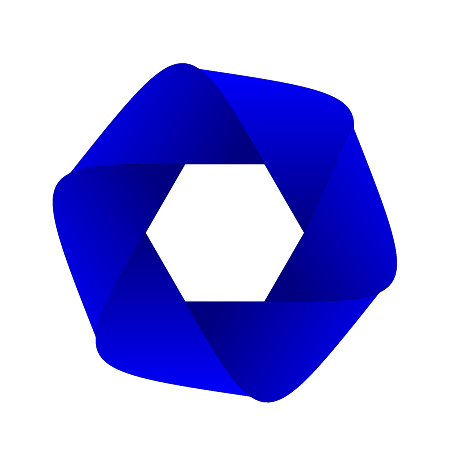
\begin{tikzpicture}[top color=black!50!blue,bottom color=blue]
\node[my polygon=6] (a){};
\foreach \x[remember=\x as \xp (initially 6)] in {1,...,6}{ % use `in {1}` to see the edge
  \fill[shade,shading angle={60*(\x+2)}] (a.corner \xp)
     ..controls ++(60*\x:2cm) .. 
     ([shift={({60*(\x+1)+6}:1.5cm)}]a.corner \x) 
     -- (a.corner \x);% Come back such that shading doesn't leak
}
\end{tikzpicture}
\end{document}